%% Copyright 2007, 2008, 2009 Elsevier Ltd

\documentclass[preprint,12pt]{elsarticle}

\usepackage{verbatim} % comentarios
\usepackage{epsfig}
\usepackage{amssymb} 

\usepackage{mathtools}

\usepackage{lineno}

\usepackage{tikz}        %permite rellenar las figuras (circulos)
\usepackage{etoolbox}
%\usepackage[backend=biber,citestyle=authoryear]{biblatex}

%\usepackage{epstopdf}


\usepackage[caption=false]{subfig}

\begin{document}

\newcommand*{\hwplotB}{\raisebox{3pt}{\tikz{\draw[red,dashed,line 
width=3.2pt](0,0) -- 
(5mm,0);}}}

\newrobustcmd*{\mydiamond}[1]{\tikz{\filldraw[black,fill=#1] (0,0) -- 
(0.1cm,0.2cm) --
(0.2cm,0) -- (0.1cm,-0.2cm);}}

\newrobustcmd*{\mytriangleleft}[1]{\tikz{\filldraw[black,fill=#1] (0,0.15cm) -- 
(-0.3cm,0) -- (0,-0.15cm);}}
\definecolor{Blue}{cmyk}{1.,1.,0,0} 

\begin{frontmatter}


\title{Effects of the body force on the evacuation dynamics}


\begin{abstract}

\end{abstract}

\begin{keyword}

Pedestrian Dynamics \sep Social Force Model \sep Body Force


\PACS 45.70.Vn \sep 89.65.Lm

\end{keyword}

\end{frontmatter}

%\linenumbers

\section{\label{introduction}Introduction}

The Social Force Model (SFM) addresses two physical forces as 
\textit{essential}: the ``body force'' and the ``sliding friction''. Both are 
inspired by granular interactions and were claimed to be necessary  
for attaining the particular effects in panicking crowds \cite{helbing_2000}. 
The ``sliding friction'' actually proved to be an essential feature of the 
``faster-is-slower'' effect, although the role of the ``body force'' appears, 
at a first instance, not so clear \cite{dorso_2005,dorso_2007,dorso_2011}. \\ 

The existence of a ``body force'' in the context of highly dense crowds (say, 5 
to 10$\,$people/m$^2$) is a commonsense matter \cite{henein_2007,fruin_1993}. 
Researchers, however, question the numerical setting for this force in 
the SFM context \cite{lakoba_2005}. As a matter of fact, the usual setting by 
Helbing prevents the overlapping among pedestrians, but it is known to 
accomplish artificially high force levels 
\cite{helbing_2000,lakoba_2005,langston_2006,lin_2017}. The force estimates 
from the SFM appear to be remarkably higher with respect to the reported real 
life data (say, an order of magnitude). The crowd motion simulations, however, 
present quite realistic results \cite{lakoba_2005,langston_2006,dorso_2017}. 
The 
point seems to be that the SFM focuses on the ``incoordination phenomenon'' due 
to clogging, missing the ``individualistic'' perspective  of single pedestrians 
or very small groups \cite{helbing_2000,henein_2007,narain_2009}.  \\ 

Many researchers realized that modifying the SFM may (partially) surpass the 
misleading parameter setting. It was proposed that the pedestrians' 
psychological force (say, the ``social force'') should be suppressed in the 
context of highly dense crowds 
\cite{pelechano_2007,moussaid_2011,alonso_2014,bottinelli_2017}, or smoothly 
quenched according to the crowd density \cite{song_2019}. The authors in 
Refs.~\cite{kabalan_2017,jebrane_2019} further proposed a rigid body model in 
order to completely avoid the overlapping phenomenon. This perspective 
dismisses 
any connection to a ``sliding friction''. Conversely, other authors tried to 
limit the pedestrians acceleration by introducing ``static friction'' between 
the pedestrians and the floor \cite{wang_2019}. This kind of friction, however, 
reduces the effective willings of the pedestrians.  \\  

A meaningful (individualistic) numerical setting appears not available yet (to 
our knowledge). The reason is that different numerical settings can lead to 
the same crowd dynamics. Actually, only a small set of dimensionless 
``numbers'' control the crowd dynamics \cite{dorso_2019}. These are similar to 
those encountered in other active matter systems (P\'eclet number, etc.)  
\cite{marchetti_2014}. We may hypothesize that while the dimensionless 
``numbers'' provide some kind of control on the ``incoordination phenomenon'' 
in 
crowds, only a few numerical settings can attain an ``individualistic'' 
meaning. 
 \\

The numerical setting for the ``faster is slower'' effect presented by 
Helbing and co-workers is somewhat cumbersome 
Ref.~\cite{helbing_2000,dorso_2017,dorso_2019}. Although a single 
parameter (say, the desired velocity $v_d$) is numerically varied to 
explain the phenomenon, the researcher looses sight of the dimensionless 
``numbers'' that truly control the crowd dynamics. The setting in 
Ref.~\cite{helbing_2000} also misses the ``faster is faster'' effect reported 
to occur at very high pedestrian densities \cite{dorso_2017,haghani_2019}. 
Alternatively, the empirical fundamental diagram raises as a point of reference 
for the SFM control parameters \cite{helbing_2007,dorso_2017}. \\

The fundamental diagram exhibits the flux behavior for either low dense crowds 
(with seldom contacts between pedestrians) and highly dense crowds (dominated 
by 
body forces and sliding friction). The latter usually experiences a flux 
slowing 
down, but other behaviors are also possible \cite{helbing_2007,lohner_2018}. In 
light of our previous hypothesis, we may suspect that the  modeling of the 
``flux slowing down'' within the context of the SFM will require the proper 
setting of the (dimensionless) controlling parameters. We examined this working 
hypothesis in Ref.~\cite{dorso_2019}, but limiting the parameter exploration to 
the sliding friction, disregarding the body force. \\

We now widen the investigation on the parameter settings to include the one 
associated to the body force. We will focus on the complex interplay between 
the body force and the sliding friction among pedestrians. Recall that the 
interplay dynamics is not directly controlled by the numerical setting, but 
through dimensionless ``numbers'', where the model parameters appear mixed 
between each other. Thus, this step up offers a challenge to the 
``individualistic'' meaning of the parameter's setting. \\  


The investigation is organized as follows. We first recall the available 
experimental values on the body force and the sliding friction (see Section 
\ref{experimental}). Secondly, we introduce the reduced-in-units SFM and the 
three dimensionless numbers that control the crowd dynamics (see Section 
\ref{background}). We present our numerical simulations in Section 
\ref{results}. For the sake of clarity, this Section is 
separated into two major parts: the bottleneck scenario and the corridor 
scenario in Sections \ref{bottleneck} and \ref{corridor}, respectively. 
Section \ref{discussion} opens a detailed discussion raising from of the results 
in Section \ref{results}. The last Section closes the investigation with our 
main conclusions.

\section{\label{experimental}Experimental background}

The complex behavior of pedestrians feature either his (her) feelings and 
the environmental conditions. The former is expressed, for example, by his 
(her) moving ``attitude'' (say, self-assuredness). The latter brings out the 
observed separation between pedestrians. Also, the ``contacts'' between 
individuals address some kind of ``unwanted'' slowing down. All these 
observed patterns are commonly quantified in the literature into a set of 
characteristic  parameters. The experimental meaning of these parameters is as 
follows.

\begin{itemize}
\item[(i)] The walking attitude of a pedestrian may appear somewhat 
``assertive'' if he (she) reacts actively to unexpected behaviors 
\cite{lakoba_2005,helbing_1995}. The smaller the reaction time, the more 
assertive or aggresive observed posture. The associated parameter to this 
behavior is the relaxation or characteristic time $\tau$ 
\cite{johansson_2009,helbing_2000}. 

\item[(ii)] Despite the reactive attitude $\tau$, the pedestrian addresses a 
``free'' (undisturbed) walking speed $v_0$. This speed expresses his (her) 
motivation or intention to reach a certain destination (as comfortable as 
possible). Observations commonly associate $0.6\,$m/s, $1\,$m/s or $1.5\,$m/s 
to relaxed, normal or nervous walking speeds, respectively  
\cite{helbing_1995,helbing_2000,li_2015}. 

\item[(iii)] The walking speed of pedestrians appears to be lower in a 
crowded walkway with respect to their usually expected ``free'' walking speeds 
\cite{weidmann_1992,lakoba_2005}. Pedestrians tend to reduce their speed within 
crowded environments because they perceive not enough space for taking a 
step  \cite{johansson_2009}. This (perceived) step distance is therefore an 
influential parameter on the pedestrians behavior. It is known as the 
characteristic length $B$. 

\item[(iv)] Physical interactions occur in very crowded environments. The 
``body force''  and ``sliding friction'' can be introduced straight forward. 
This will be done in Section \ref{background}. But it is worth noting that 
both are associated to the moving difficulties (say, slowing down and 
obstructions) observed in contacting pedestrians. 

\end{itemize}


Table~\ref{table_data} shows a few empirical figures for the most common 
parameters. More data is available throughout the literature (see, for example, 
Refs.~\cite{hoogendoorn_2007,seyfried_2007,johansson_2007,moussaid_2009,
luber_2010,seer_2014,li_2015} ). We intentionally omitted data that assumes a 
specific mathematical model. The exhibited values should also be considered as a 
general purpose approach, since no distinction has been made on age, gender or 
cultural habits. \\

\begin{table}
\begin{tabular}{c@{\hspace{6mm}}c@{\hspace{6mm}}c@{\hspace{6mm}}c@{\hspace{6mm}}
c@{\hspace{14mm}}l}
 \hline
 $\tau$[s]   & $m$[kg]     & $v_d$[m/s]  &  $B$[m]  & $k$[kg/s$^2$] &  Refs. \\
 \hline
0.61         & ---         & 1.24 & $0.36+1.06\,v$ &  ---                 &  
 \cite{seyfried_2007} \\
0.50$^*$     & 80$^*$      & 1.34 & 0.50           &  ---                 &  
\cite{weidmann_1992,lakoba_2005}\\
---          & $67.5$      & 1.39 &  ---           &  $96.1 + 12694.1\,x$ & 
\cite{song_2019}\\
---          & $67.0$      & 1.39 &  ---           &  $97.0 + 29378.9\,x$ & 
\cite{song_2019}\\


\hline
\end{tabular}
\caption{The experimental data for the pedestrian parameters, as explained in 
Section~\ref{experimental}. The magnitude $v$ means de pedestrian velocity 
(m/s). The magnitude $x$ means the compression length (m). The upper row for 
Ref.~\cite{song_2019} corresponds data acquired in winter and the lower row to 
datas acquiquired in summer. The asterisk ($^*$) corresponds to reasonable 
estimates from the authors. }
\label{table_data}
\end{table}

A first examination of the figures in Table~\ref{table_data} shows that the 
choise $\tau\simeq0.6\,$s seems to be a reasonable estimation for the 
relaxation time, although this may vary with respect to gender or culture 
\cite{siddharth_2018}. Additionally, we confirm that normal pedestrians attain 
desired velocities around $1.3\,$m/s. \\

The reports from Refs.~\cite{seyfried_2007,weidmann_1992} do not include any 
values for the compressibility $k$ since these experiments were carried out 
under low density conditions. Notice that the minimum (perceived) step distance 
is $0.36\,$m \cite{seyfried_2007}, but the pedestrians seem to require larger 
distances when they walk faster. The commonly accepted value $B\simeq 
0.5\,$m is somewhat valid for walking speeds under $0.5\,$m/s 
\cite{seyfried_2007}. Higher walking speeds (say, $1\,$m/s) will require 
a step distance of $1.3\,$m for the pedestrians to feel that there is enough 
space to move along.     \\ 

The reported data from Ref.~\cite{song_2019} correspond to the crowded 
environment of the Beijing subway. This environment was not suitable for 
providing information on the step distance $B$, but estimates for the 
desired speed and the body compresibility could be achieved. The reported 
magnitude $k$ assesses either the clothes and the body compressibility. The 
final value, though, is linearly related to the compression $x$. \\

We measured the maximum attainable forces at the subway in Buenos Aires, 
Argentina. Our preliminary results show that pedestrians feel ``uncomfortable'' 
whenever a body force ranging from $5$ to $20\,$N is applied for at least ten 
minutes. Short lasting forces (say, less than 4 minutes) may also be perceived 
as ``uncomfortable'' for values ranging from $10$ to $30\,$N. We also recorded body 
forces up to $60\,$N during very short ``hits''. The comparison with the 
fittings provided by Ref.~\cite{song_2019} shows that these magnitudes 
accomplish densities around 5 people/m$^2$.     \\    

The maximum (realistic) compressions may be computed from the relation 
$F=k(x)\,x$ and the compressibility $k(x)$ reported in Table~\ref{table_data}. 
An ``uncomfortable'' body force of $30\,$N can address compressions in the 
range of $0.030-0.055\,$m. Also, a ``hitting'' force of $60\,$N can address 
compressions between $0.045$ and $0.065\,$m. Thus, according to 
Table~\ref{table_data}, we may expect experimental values for $k(x)$ up to 
$1000\,$kg/s$^2$ (for $F=30\,$N), or, up to $1400\,$kg/s$^2$ (for $F=60\,$N). \\

Besides, no realiable values for the sliding friction $\kappa$ appears to be 
available in the literature (to our knowledge). We may pressume, however, that 
the sliding friction approaches a fraction of the body force. We will come back 
to this issue in Section~\ref{background}. \\


\section{\label{background}Theoretical background}

\subsection{\label{sfm}The Social Force Model}

The Social Force Model (SFM) provides the necessary framework for simulating 
the collective dynamics of self-driven particles (\textit{i.e.} pedestrians). 
The pedestrians are considered to follow an equation of motion involving 
either ``socio-psychological'' forces and physical forces (say, granular 
forces). The equation of motion for any pedestrian $i$ (of mass $m_i$) reads

\begin{equation}
 m_i\,\displaystyle\frac{d\mathbf{v}_i}{dt}=\mathbf{f}_d^{(i)}+
 \displaystyle\sum_{j=1}^N\mathbf{f}_s^{(ij)}+
 \displaystyle\sum_{j=1}^N\mathbf{f}_g^{(ij)}\label{eqn_motion}
\end{equation}

\noindent where the subscript $j$ corrresponds to any neighboring pedestrian or 
the walls. The three forces $\mathbf{f}_d$, $\mathbf{f}_s$ and $\mathbf{f}_g$ 
are different in nature. The desire force $\mathbf{f}_d$ represents the 
acceleration (or deceleration) of the pedestrian due to his (her) own willings. 
The social force $\mathbf{f}_s$, intead, describes the tendency of the 
pedestrians to stay away from each other. The granular force $\mathbf{f}_g$ 
stands for either the sliding friction and the compression between 
pedestrians. \\

Notice that these forces are supposed to influence the behavior of the 
pedestrians in a similar fashion as mentioned in Section~\ref{experimental}. 
Thus, the set of (empirical) parameters described in Section~\ref{experimental} 
is expected to be also present in the SFM. These will appear in connection to 
the forces, although their meaning may be somewhat different. \\   

The pedestrians' own willing is modeled by the desire force $\mathbf{f}_d$. 
This force stands for the acceleration (deceleration) required to reach a 
certain position at the desired walking speed $v_d$. This involves, however, a 
personal attitude that makes him (her) appear more or less ``assertive''. As 
mentioned in Section~\ref{experimental}, the reaction time $\tau$  attains for 
this attitude. Thus, the desire force is modeled as follows

\begin{equation}
\mathbf{f}_d^{(i)}=m\,\displaystyle\frac{v_d^{(i)}\,
\hat{\mathbf{e}}_d^{(i)}(t)-
 \mathbf{v}^{(i)}(t)}{\tau}
\end{equation}


\noindent where $\hat{\mathbf{e}}(t)$ represents the unit vector pointing to 
the target position. $\mathbf{v}(t)$ stands for the pedestrian velocity at time 
$t$. \\

The tendency of any individual to preserve his (her) ``private sphere'' is 
accomplished by the social force $\mathbf{f}_s$. This force is expected to 
prevent the pedestrians from getting too close to each other (or to the walls) 
in a crowded environment. If he (she) perceives that there is not enough space 
to move, he (she) will decelerate or even move back. The model for this kind of 
``socio-psychological'' behavior is as follows

\begin{equation}
 \mathbf{f}_s^{(i)}=A\,e^{(R_{ij}-r_{ij})/B}\,\hat{\mathbf{n}}_{ij}
 \label{eqn_social}
\end{equation}

\noindent where $r_{ij}$ means the distance between the center of mass of the 
pedestrians $i$ and $j$, and $R_{ij}=R_i+R_j$ is the sum of the pedestrians 
radius. The unit vector $\hat{\mathbf{n}}_{ij}$ points from pedestrian $j$ to 
pedestrian $i$, meaning a repulsive interaction.\\ 

The net distance $|R_{ij}-r_{ij}|$ scales to the parameter $B$ in the 
expression (\ref{eqn_social}). This parameter plays the role of a fall-off 
length within the model, and thus, it may be somewhat connected to the 
(perceived) step distance mentioned in Section~\ref{experimental}. The 
parameter $A$, however, does not provide any direct link to other parameters 
mentioned there. \\    

The granular force (say, the sliding friction plus the body force) attain to 
the moving difficulties encountered in very crowded environments. The 
expression for the granular force is has been borrowed from other granular 
matter fields, as follows

\begin{equation}
 \mathbf{f}_g^{(ij)}=\kappa\,g(R_{ij}-r_{ij})\,
(\Delta\mathbf{v}^{(ij)}\cdot\hat{\mathbf{t}}_{ij})\,\hat{\mathbf{t}}_{ij}+
k\,g(R_{ij}-r_{ij})\,
\,\hat{\mathbf{n}}_{ij}\label{eqn_friction}
\end{equation}

\noindent where $g(R_{ij}-r_{ij})$. $\Theta(R_{ij}-r_{ij})$ equals R_{ij}-r_{ij} 
if $R_{ij}>r_{ij}$ and vanished otherwise. 
$\Delta\mathbf{v}^{(ij)}\cdot\hat{\mathbf{t}}_{ij}$ represents the difference 
between the tangential velocities of the sliding bodies (or between the 
individual and the walls).    \\

The sliding friction occurs in the tangential direction while the body force 
occurs in the normal direction. Both are assumed to be linear with respect to 
the net distance between contacting pedestrians. The sliding friction is also 
linearly related to the difference between the (tangential) velocities. The 
coefficients $\kappa$ (for the sliding friction) and $k$ (for the 
body force) are supposed to be related to the areas of contact and the clothes 
material, among others. \\

We stress that the expression (\ref{eqn_friction}) assumes fixed values for 
$\kappa$ and $k$. This may not be completely true according to 
Table~\ref{table_data}. The local density (and thus, the pedestrians' 
compression) may affect the compressibility parameter $k$ by more than an order 
of magnitude. We will vary $k$ (and $\kappa$) in order to explore this 
phenomenon. \\  


\subsection{\label{sfm}The parameters setting}


\begin{figure}[!htbp]
\centering
    \subfloat[]{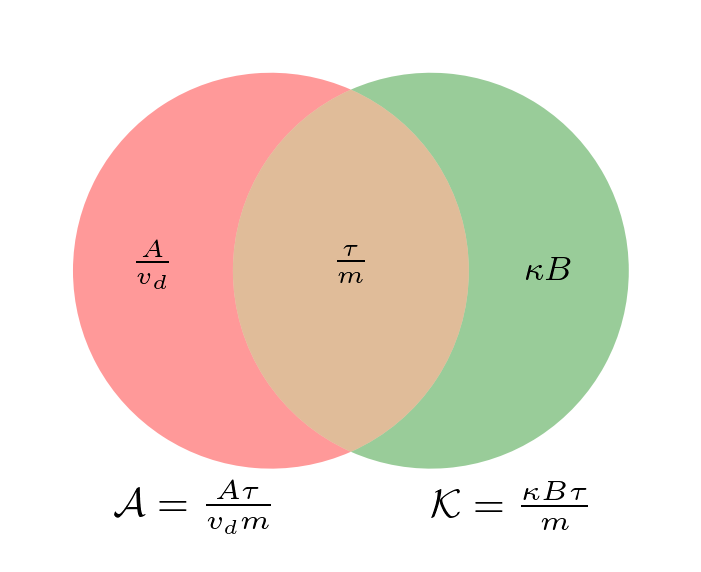
\includegraphics[width=0.45\columnwidth]{./venn_2parameters.png}\label{venn_2parameters}}\ 
    \subfloat[]{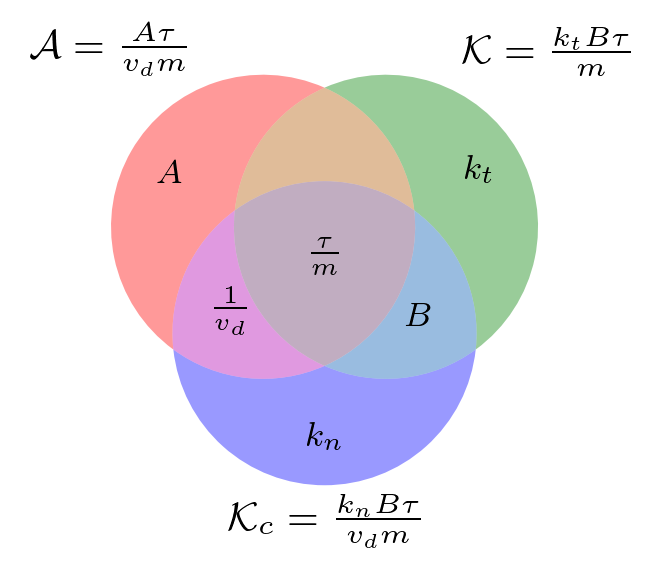
\includegraphics[width=0.45\columnwidth]{./venn_3parameters.png}\label{venn_3parameters}}\\
\caption[width=0.47\columnwidth]{}
\label{flow_density}
\end{figure}


\section{\label{results}Results}


\subsection{\label{bottleneck} Bottleneck}


In this section, we present the results corresponding to the bottleneck geometry. We show how the overall dynamic of the system changes depending on the $k$ value associated to the body force in the original SFM.\\

Fig. \ref{vd_vs_te} shows the evacuation time as a function of the pedestrian's desired velocity. The evacuation time was defined as the time until 70\% of the pedestrians left the room. The different markers correspond to different $k$ values ($i.e$ different body ``stiffness''). The crosses correspond to the Helbing original SFM parameter, the up-triangles correspond to the value measured in Ref ..., squares correspond to an absent body force and circles correspond to an extreme value of stiffness (one order of magnitude higher than the original SFM). The down triangles correspond to an intermediate value between the empirical value presented in Ref... and the chosen by Helbing in Ref...\\

There is a noticeable difference in the evacuation time depending on the $k$ value of the body force. The higher the $k$ the smaller the evacuation time, meaning that if pedestrians are stiffer, the overall speed increases (hence the evacuation time decreases).\\

The Faster-is-Faster (FIF) is the phenomenon in which under certain conditions, increasing the desired velocity yields to a reduction of the evacuation time. The Faster-is-Faster is the opposite effect (the higher $v_d$ the lower the evacuation time).  Notice that the presence of the Faster-is-Faster (FIF) effect and the Faster-is-Slower are dependent on the value of $k$. In Fig.~\ref{vd_vs_te} we can see that $k=1.2$~E5 only exhibits FIS effect for $v_d>$2~m/s. When $k=1.2$~E6, the evacuation time reduces as $v_d$ increases, meaning that only FIF is reported. The explored values of $k$ that satisfy $k \leq 6$~E4 exhibit both the FIS and the FIF effect depending on the range of desired velocities. Notice that the behavior of the case in which $k = 0$ is very similar to the case in which $k = 1.2$~E4.\\
% se puede discutir que este resultado es importante porque k=1.2E4 es un valor empirico y k=1.2E5 tambien lo es, osea que el FIF podria estar o no estar dependiendo de cual es el verdadero valor de k. Habria que chequear en unidades reducidas como queda. 
 

\begin{figure}[htbp!]
\centering
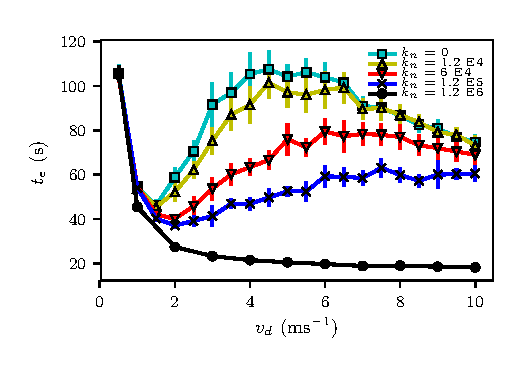
\includegraphics[width=0.7\columnwidth]
{./vd_vs_te_N225.eps}
\caption{\label{vd_vs_te}Mean evacuation time (s) vs. the pedestrian’s desired velocity (m/s) for a bottleneck. The room was 20 m x 20 m size. The door was 0.92 m width. Mean values were computed from 10 evacuation processes. 225 pedestrians were initially placed in a square lattice with a random initial velocity. Each process was finished when 158 pedestrians left the room. The different symbols indicate the $k$ value corresponding to the body force (see the label). }
\end{figure}


Network analysis is a set of techniques that characterize the structures in a graph. We defined the graph of contacts among individuals. In this graph, each node represents a pedestrian and the link between a pair of nodes is settled if the pedestrians are in physical contact ($i.e.$ $r_{ij}<d_{ij}$).\\

Fig.~\ref{degree_vd} shows the mean degree of the contact graph as a function of the desired velocity. The degree of a node is defined as the amount of edges assigned to the node. This means, the number of pedestrians that are in physical contact with a given pedestrian. The mean degree is the average of the degree over all the nodes (pedestrians) and over the whole sampled time (from the time the system reaches the stationary state to the end of the simulation).\\

Increasing $v_d$ increases the mean degree in all the cases. This happens because increasing $v_d$ produces higher densities that force individuals to touch each other. For a given $v_d$ the mean degree reduces as the $k$ value increases. In other words, the stiffer the pedestrians the less they touch each other. We will later discuss that this phenomenon is restricted to the bottleneck geometry that cannot be extrapolated to the corridor geometry.\\

Fig.~\ref{overlap_vd} shows the overlap as a function of $v_d$. The overlap is defined as $d_{ij}-r_{ij}$ where $d_{ij}$ is the sum of radius of particle $i$ and particle $j$ and $r_{ij}$  is the distance between both particles. In the range $v_d \geq 2$~m/s we can see that increasing $v_d$ increases the overlap (for all the $k$ values studied). For a given $v_d$, the overlap increases as the $k$ value decreases. Reducing $k$ means reducing the normal body force which allows a greater invasion of the personal space of the individuals.\\  


\begin{figure}[!htbp]
\centering
    \subfloat[]{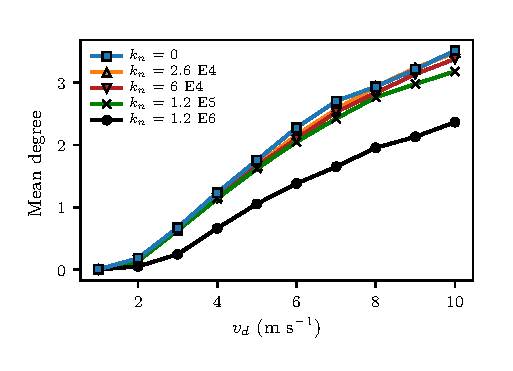
\includegraphics[width=0.45\columnwidth]{./degree_vs_vd_multi_kn.eps}\label{degree_vd}}\ 
    \subfloat[]{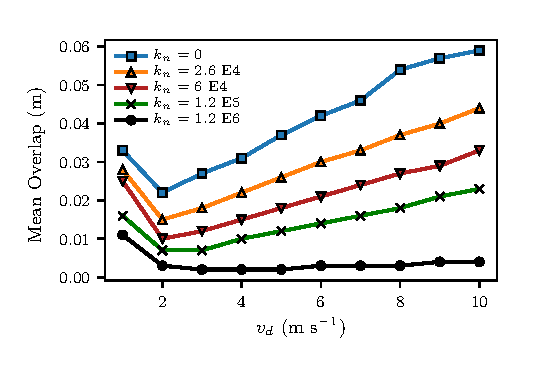
\includegraphics[width=0.45\columnwidth]{./overlap_vs_vd_multi_kn.eps}\label{overlap_vd}}\\
\caption[width=0.47\columnwidth]{(a) Mean degree as a function of the pedestrian’s desired velocity (m/s). (b) Mean overlap as a function of the pedestrian’s desired velocity (m/s). Each symbol indicates the $k$ value corresponding to the body force (see the labels). The data corresponds to a bottleneck with periodic boundary conditions (re-injecting pedestrians). The average was taken every two seconds once the crowd reaches the stationary state ($t=$20~s) until the end of the simulation ($t=$110~s).}
\label{degree_overlap_vd}
\end{figure}



\begin{figure}[!htbp]
\centering
    \subfloat[]{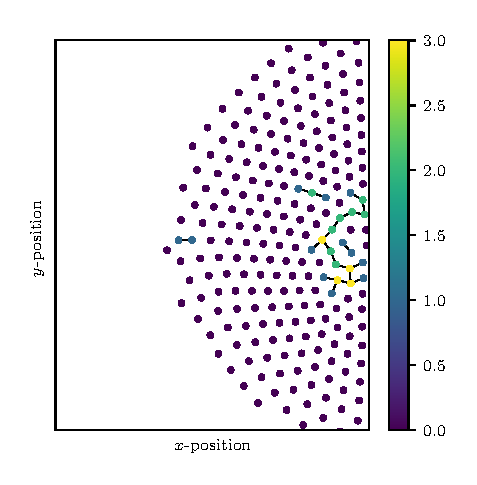
\includegraphics[width=0.45\columnwidth]{./network_vd2_kn0.eps}\label{flow_density_nocomp}}\ 
    \subfloat[]{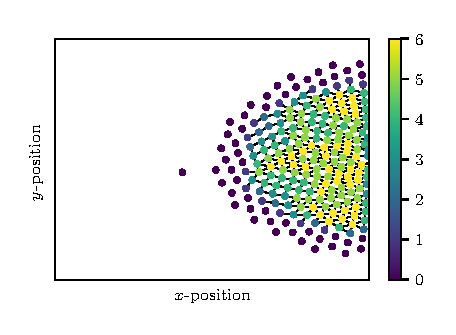
\includegraphics[width=0.45\columnwidth]{./network_vd10_kn0.eps}\label{flow_density_comp}}\\
        \subfloat[]{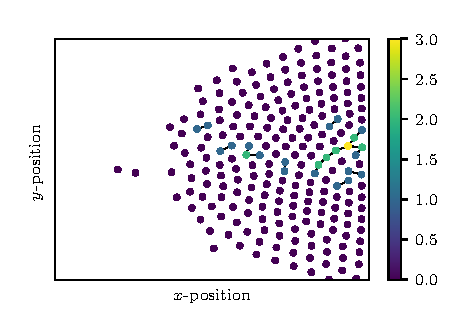
\includegraphics[width=0.45\columnwidth]{./network_vd2_kn120000.eps}\label{flow_density_nocomp}}\ 
    \subfloat[]{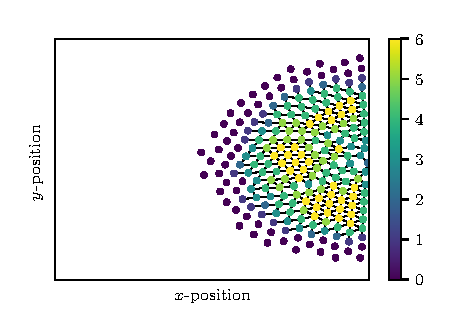
\includegraphics[width=0.45\columnwidth]{./network_vd10_kn120000.eps}\label{flow_density_comp}}\\
\caption[width=0.47\columnwidth]{}
\label{flow_density}
\end{figure}



\subsection{\label{corridor} Corridor}


\begin{figure}[!htbp]
\centering
    \subfloat[]{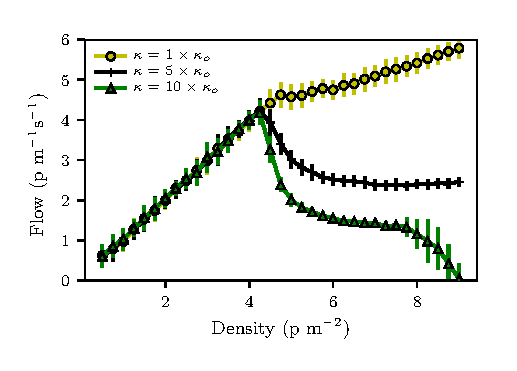
\includegraphics[width=0.45\columnwidth]{./flow-density_multifric_nobodyforce.eps}\label{flow_density_nocomp}}\ 
    \subfloat[]{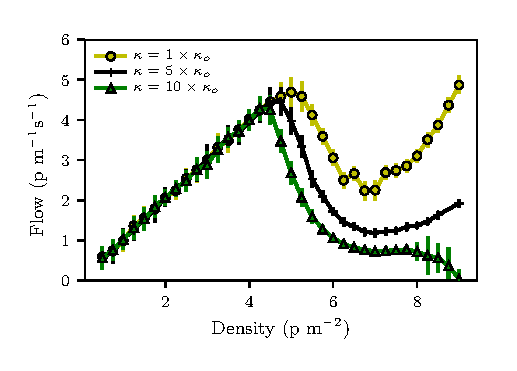
\includegraphics[width=0.45\columnwidth]{./flow-density_multifric_bodyforce.eps}\label{flow_density_comp}}\\
\caption[width=0.47\columnwidth]{}
\label{flow_density}
\end{figure}

\begin{figure}[!htbp]
\centering
    \subfloat[]{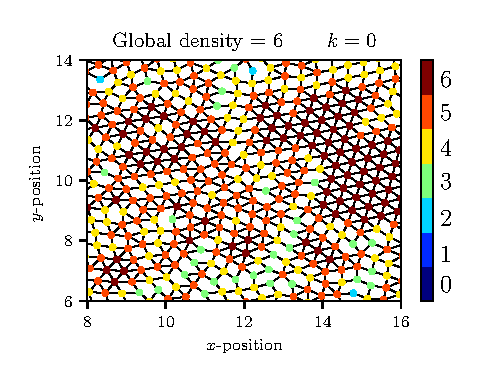
\includegraphics[width=0.45\columnwidth]{./network_d6_kn0.eps}\label{network_d6_kn0}}\ 
    \subfloat[]{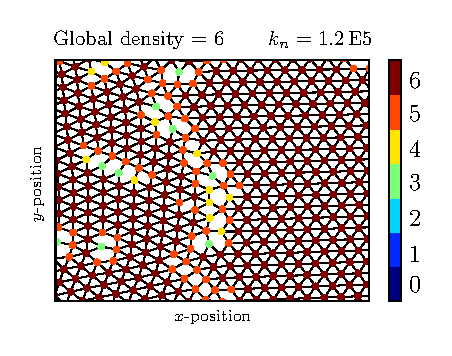
\includegraphics[width=0.45\columnwidth]{./network_d6_knE5.eps}\label{network_d6_knE5}}\\
\caption[width=0.47\columnwidth]{}
\label{network_corridor}
\end{figure}


\begin{figure}[!htbp]
\centering
    \subfloat[]{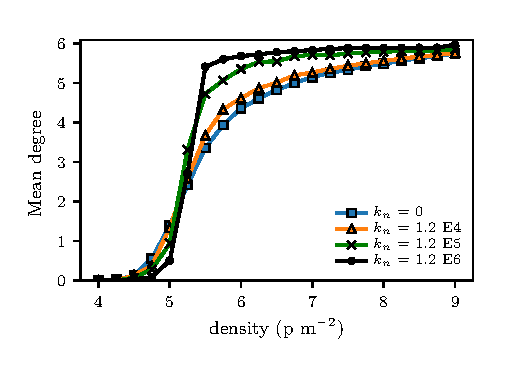
\includegraphics[width=0.45\columnwidth]{./degree_vs_dens_multi_kn.eps}\label{degree_dens}}\ 
    \subfloat[]{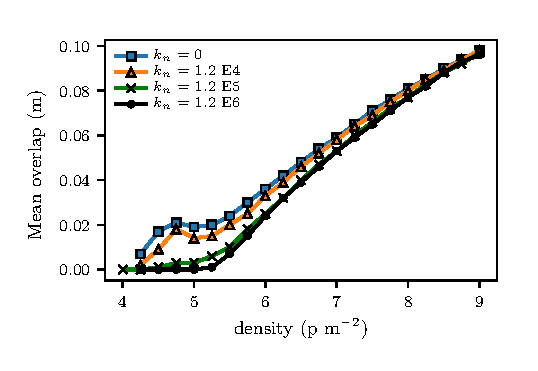
\includegraphics[width=0.45\columnwidth]{./overlap_vs_dens_multi_kn.eps}\label{overlap_dens}}\\
\caption[width=0.47\columnwidth]{}
\label{network_corridor}
\end{figure}



\begin{figure}[htbp!]
\centering
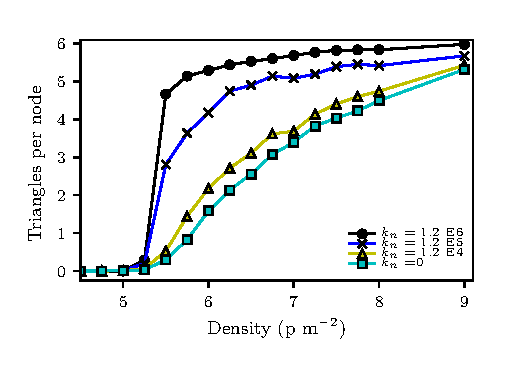
\includegraphics[width=0.7\columnwidth]
{./triangles.eps}
\caption{\label{} }
\end{figure}




\subsection{\label{reduced-in-units} Reduced-in-units equation of motion}


\section{\label{discussion}Discussion}



\section{\label{conclusions}Conclusions}

\section*{Acknowledgments}
This work was supported by the National Scientific and Technical 
Research Council (spanish: Consejo Nacional de Investigaciones Cient\'\i ficas 
y T\'ecnicas - CONICET, Argentina) grant Programaci\'on Cient\'\i fica 2018 (UBACYT) Number 20020170100628BA.

\appendix



%/////////////////////////////////////////////////
%\begin{thebibliography}{10}
%\expandafter\ifx\csname url\endcsname\relax
%  \def\url#1{\texttt{#1}}\fi
%\expandafter\ifx\csname urlprefix\endcsname\relax\def\urlprefix{URL }\fi
%\expandafter\ifx\csname href\endcsname\relax
%  \def\href#1#2{#2} \def\path#1{#1}\fi

%\bibitem{helbing3}
%Helbing, D., Johansson, A., and Al-Abideen, H. Z., 2007. ``Dynamics of crowd 
%disasters: An empirical study." Physical review E 75 (4), 046109.
%{\path{https://doi.org/10.1103/PhysRevE.75.046109}}

%\end{thebibliography}

\bibliographystyle{unsrt}
\bibliography{paper}% Produces the bibliography via BibTeX.

\end{document}
\endinput

